\DomainHeader{Debugging and Troubleshooting}{11\%}

\begin{Objectives}
  \item Recognize when \texttt{SdfChangeBlock} helps performance.
  \item Diagnose why opinions do not take effect on a composed stage.
  \item Resolve asset-management/path issues.
  \item Understand causes of unexpected visual results.
  \item Use diagnostics/profiling: TfDebug, diagnostic delegates, Trace,
        TfMallocTag, etc.
\end{Objectives}

\begin{Resources}
  \item Tutorials: \href{https://openusd.org/release/tut_inspect_and_author_props.html}{Inspecting and Authoring Properties}; \href{https://openusd.org/release/tut_traversing_stage.html}{Traversing a Stage}
  \item Tooling: \href{https://openusd.org/release/toolset.html#usdview}{\texttt{usdview}}
        (\href{https://docs.omniverse.nvidia.com/usd/latest/usdview/panel_composition.html#layer-stack}{Layer Stack / Composition tabs}),
        \href{https://openusd.org/release/toolset.html#usdcat}{\texttt{usdcat}}
  \item Technical references: USD FAQ \href{https://openusd.org/release/usdfaq.html#what-s-the-difference-between-an-over-and-a-typeless-def}{``Over vs Typeless Def''};
        \href{https://openusd.org/release/maxperf.html}{Maximizing USD Performance}
  \item OpenUSD API: \href{https://openusd.org/release/api/class_usd_property.html}{GetPropertyStack};
        \href{https://openusd.org/release/api/class_usd_stage.html}{UsdStage::MuteLayer};
        \href{https://openusd.org/release/api/class_usd_utils_coalescing_diagnostic_delegate.html}{UsdUtilsCoalescingDiagnosticDelegate};
        \href{https://openusd.org/release/api/class_sdf_change_block.html}{SdfChangeBlock}
\end{Resources}

\CheatSheetTitle
\begin{itemize}[leftmargin=*]
  \item \textbf{The three questions}, in order: Is my edit landing in the
        layer I think (edit target)? Is a stronger opinion winning (LIVRPS)?
        Is the prim composed at all (payload loaded, reference resolved,
        variant selected, \texttt{active})?\index{edit target}
  \item \textbf{Provenance tool \#1}:
        \texttt{attr.GetPropertyStack(time)} --- every opinion for a
        property, strongest first, with its layer.\index{GetPropertyStack}
  \item \textbf{Bisection tool \#1}: \texttt{stage.MuteLayer()} --- pull
        layers out of composition one at a time until the symptom
        disappears.\index{muting layers}
  \item \textbf{usdview} shows the same story interactively: Layer Stack and
        Composition tabs (see the Composition chapter's screenshot).
  \item \textbf{SdfChangeBlock}: batch many small authoring edits into one
        recomposition --- the fix for ``my exporter spends all its time in
        change processing''.\index{SdfChangeBlock}
  \item \textbf{TfDebug}: hundreds of runtime switches
        (\texttt{TF\_DEBUG=PLUG\_*}, \texttt{AR\_*}, \texttt{PCP\_*}) that
        print what plugins, resolvers, and composition are doing.\index{TfDebug}
  \item \textbf{Silence is a lie}: warnings on stderr --- unresolved assets,
        missing \texttt{defaultPrim} --- are composition errors in disguise;
        make pipelines fail on them.
\end{itemize}

\section{Core Concepts}

\subsection{Reproduce small, then interrogate}\label{sec:dbg-repro}\objref{6.2}
Every composition mystery shrinks to a few layers. This chapter's repro ---
one definition, one override, one stack:

\begin{lstlisting}
#usda 1.0
def Sphere "Ball" {
    double radius = 1
}
\end{lstlisting}

\begin{lstlisting}
#usda 1.0
over "Ball" {
    double radius = 3
}
\end{lstlisting}

\begin{lstlisting}
#usda 1.0
(
    subLayers = [@./lite.usda@, @./base.usda@]
)
\end{lstlisting}

\subsection{Who wins, and from where}\label{sec:dbg-stack}\objref{6.2}
The single most useful debugging call in USD answers ``where did this value
come from?'' --- every authored opinion for a property, strongest first:

\begin{lstlisting}[language=Python]
from pxr import Usd

stage = Usd.Stage.Open("shot.usda")
attr = stage.GetPrimAtPath("/Ball").GetAttribute("radius")
print(attr.Get())   # 3.0
for spec in attr.GetPropertyStack(Usd.TimeCode.Default()):
    print(spec.layer.GetDisplayName(), spec.default)
# lite.usda 3.0   <-- strongest first: this one wins
# base.usda 1.0
\end{lstlisting}

\noindent This is the scripted twin of usdview's Layer Stack tab ---
Figure~\ref{fig:layerstack} is the same investigation done interactively:
select the prim, open \emph{Layer Stack}, read the opinions strongest-first.
Same workflow for whole prims: \texttt{prim.GetPrimStack()}.

\begin{figure}[ht]
  \centering
  \begin{tikzpicture}
    \node[anchor=south west, inner sep=0] (img)
      {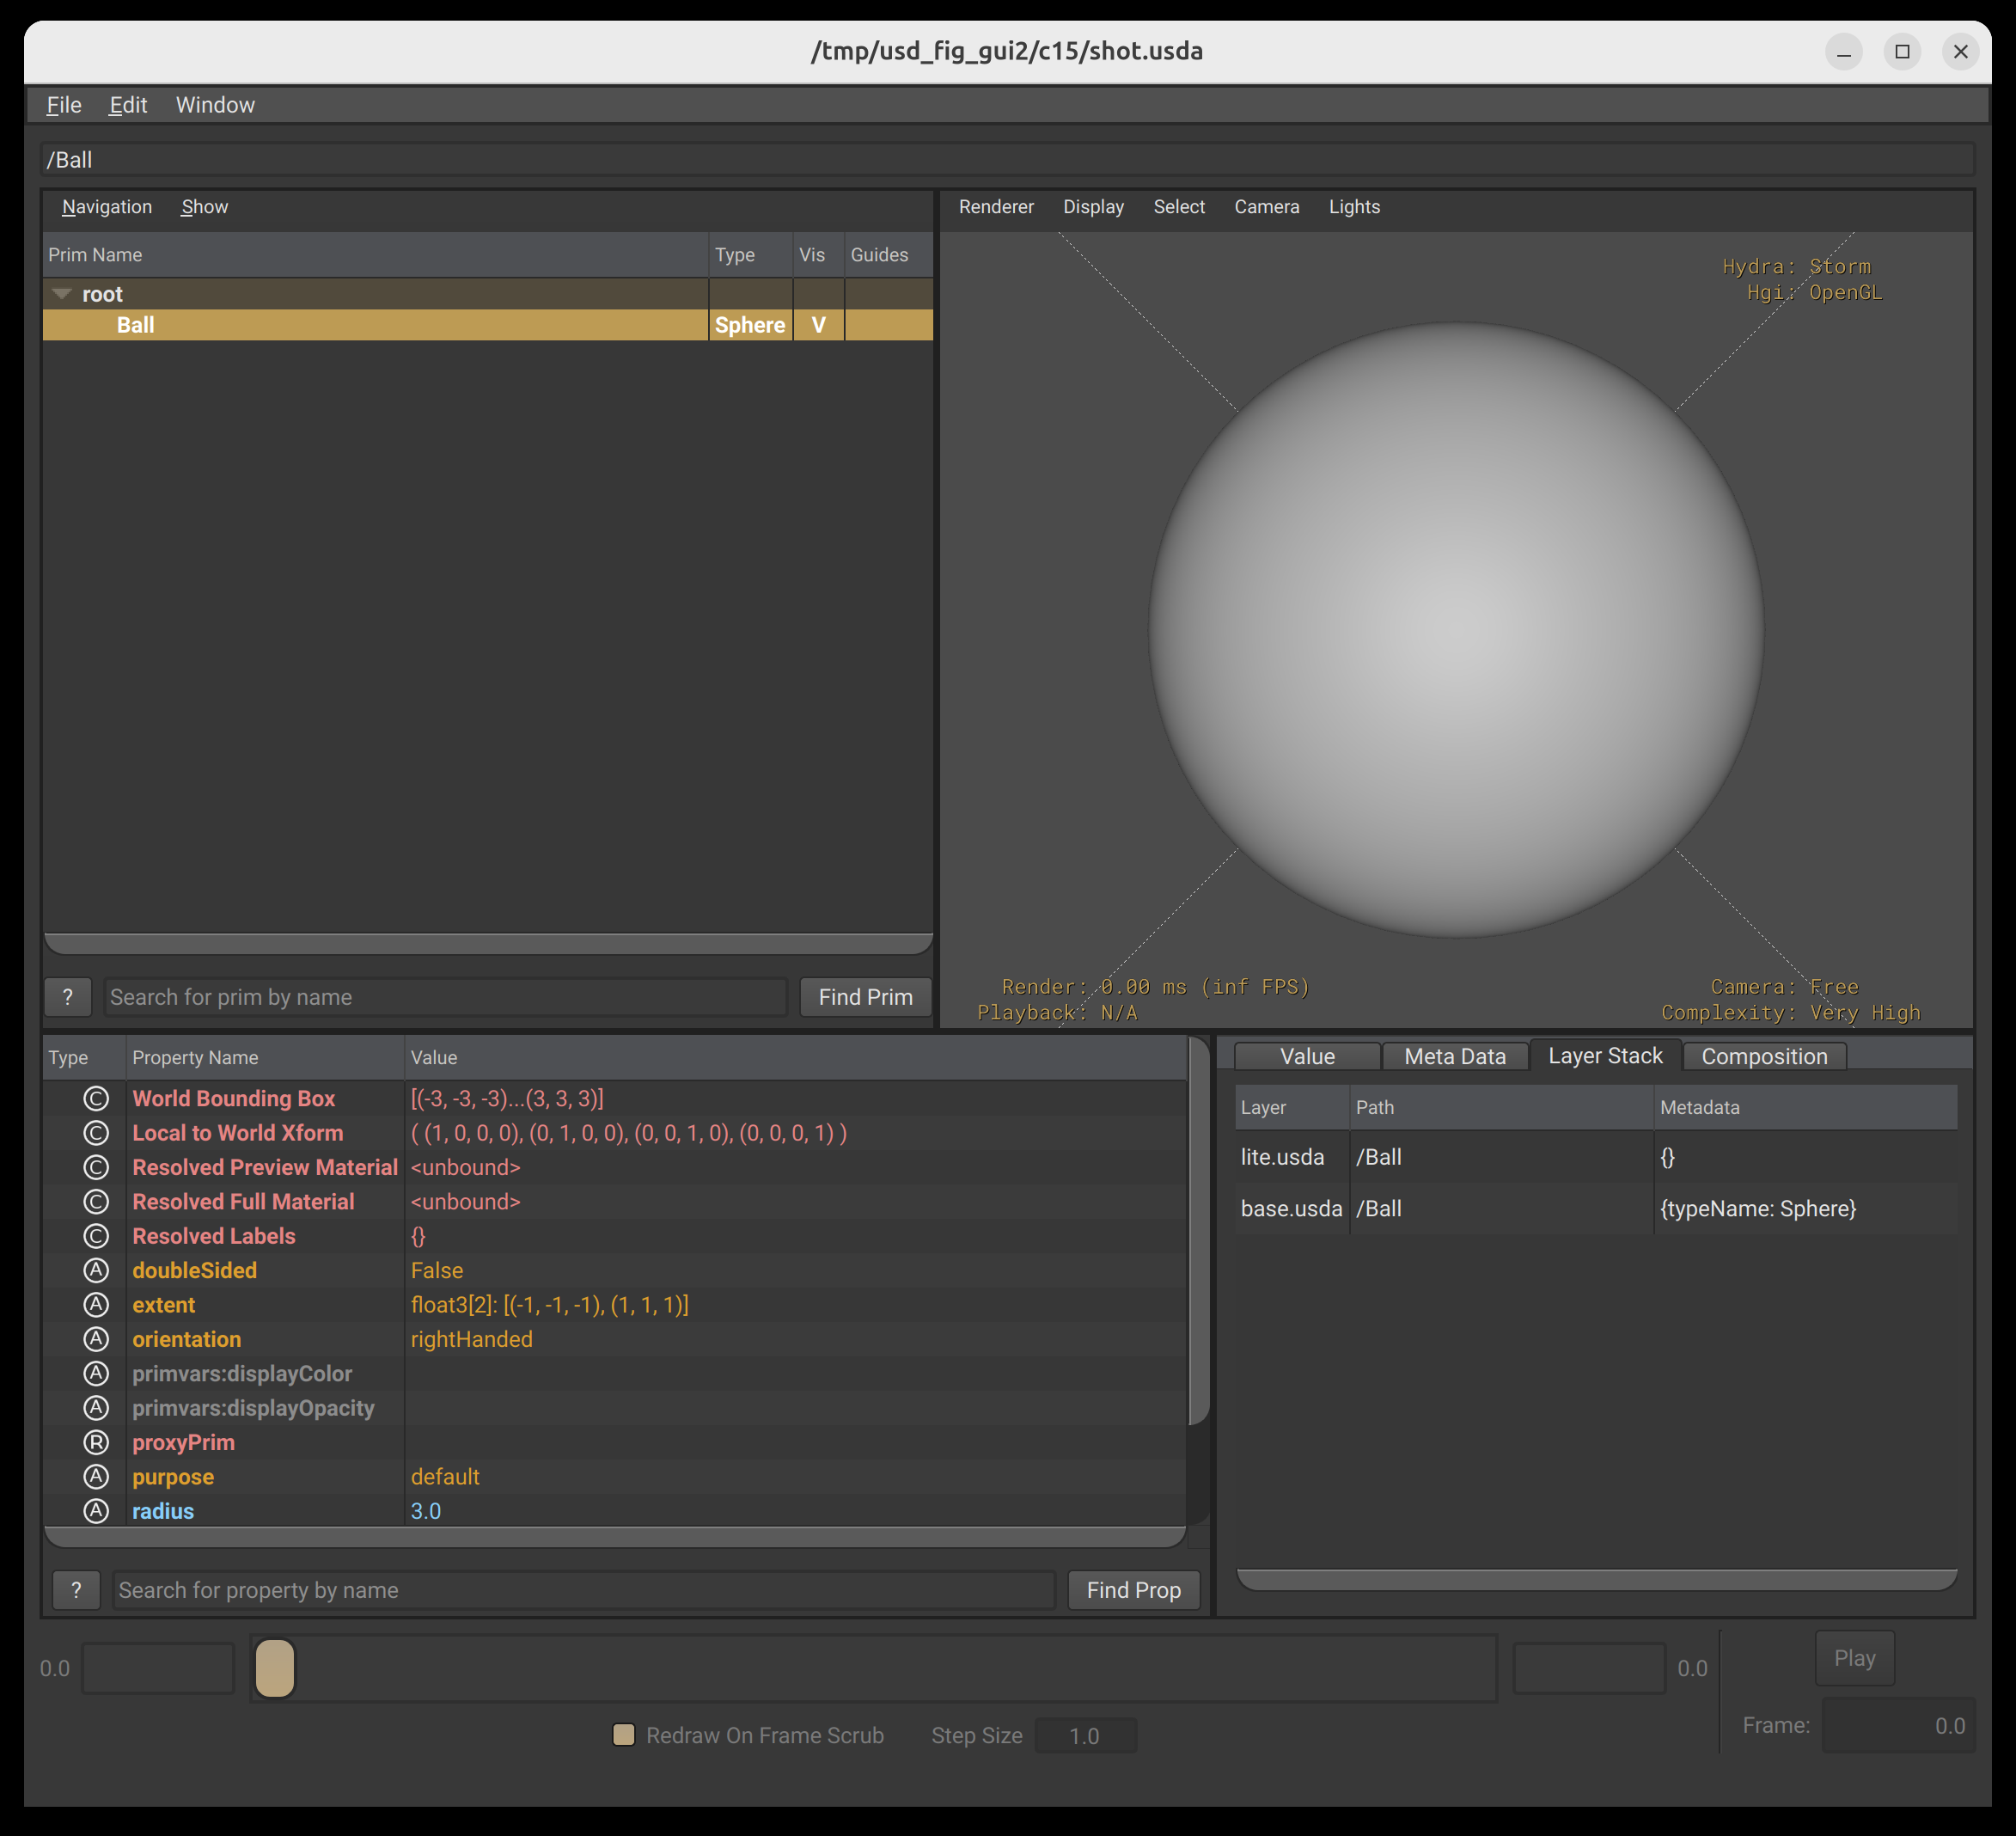
\includegraphics[width=0.95\linewidth]{figures/c15_usdview_layerstack.png}};
    \begin{scope}[x={(img.south east)}, y={(img.north west)}]
      \node[notetext, draw=arcVar, fill=white, rounded corners=1pt,
            text width=0.26\linewidth, align=left] (tab) at (0.46,0.50)
        {the \emph{Layer Stack} tab: every layer with an opinion on the
         selection};
      \draw[varArc] (tab.east) -- (0.755,0.43);
      \node[notetext, draw=usdgreen!60!black, fill=white, rounded corners=1pt,
            text width=0.26\linewidth, align=left] (rows) at (0.46,0.26)
        {\texttt{lite.usda} above \texttt{base.usda} --- strongest first,
         matching \texttt{GetPropertyStack}};
      \draw[subArc] (rows.east) -- (0.64,0.36);
    \end{scope}
  \end{tikzpicture}
  \caption{usdview on this chapter's repro with \texttt{/Ball} selected. The
  Layer Stack tab lists both contributing layers strongest-first; the
  property panel shows the winning \texttt{radius = 3.0}.}
  \label{fig:layerstack}
\end{figure}

\begin{ExamTip}
``Why doesn't my opinion take effect?'' has exactly four endings: a stronger
opinion (read the property stack top-down), the edit landed in the wrong
layer (check the edit target), the prim isn't fully composed (payload
unloaded, broken reference, wrong variant, \texttt{active = false}), or the
value never reached this property at all (typo: \texttt{over} on the wrong
path silently authors nothing useful --- see the ``over vs typeless def''
FAQ).
\end{ExamTip}

\subsection{Bisection: mute layers until the bug leaves}\label{sec:dbg-mute}\objref{6.2, 6.3}
\index{muting layers}When the property stack is deep, stop reading and start
cutting --- muting removes a layer from composition without touching files:

\begin{lstlisting}[language=Python]
from pxr import Sdf, Usd

stage = Usd.Stage.Open("shot.usda")
radius = stage.GetPrimAtPath("/Ball").GetAttribute("radius")
print(radius.Get())                       # 3.0 -- lite.usda wins

lite = Sdf.Layer.FindOrOpen("lite.usda")  # the suspect
stage.MuteLayer(lite.identifier)
print(radius.Get())                       # 1.0 -- base.usda shows through

stage.UnmuteLayer(lite.identifier)
\end{lstlisting}

\noindent The same bisection spirit applies to the working set
(\texttt{Load}/\texttt{Unload} payloads), variant selections, and
deactivating subtrees (\texttt{SetActive(False)}) --- isolate until the
symptom names its layer.

\subsection{Performance: batch your edits}\label{sec:dbg-perf}\objref{6.1}
\index{SdfChangeBlock}Every authoring call can trigger change processing and
recomposition; tools that author thousands of opinions one-by-one spend
their life there. \texttt{SdfChangeBlock} batches Sdf-level edits into a
single notification:

\begin{lstlisting}[language=Python]
from pxr import Sdf

layer = Sdf.Layer.CreateAnonymous()
with Sdf.ChangeBlock():
    for i in range(100):
        prim = Sdf.CreatePrimInLayer(layer, f"/Props/Prop_{i:03}")
        prim.specifier = Sdf.SpecifierDef
        prim.typeName = "Xform"
print(len(layer.GetPrimAtPath("/Props").nameChildren))   # 100
\end{lstlisting}

\begin{Gotcha}
Inside a change block, work at the \emph{Sdf} level and do not read back
through Usd APIs --- composition is intentionally stale until the block
closes. The objective is literally ``recognize \emph{when} SdfChangeBlock
helps'': many small edits, one recomposition. It does not make a single big
edit faster.
\end{Gotcha}

\subsection{Diagnostics: make USD tell you}\label{sec:dbg-diag}\objref{6.5}
\index{TfDebug}USD ships with runtime debug switches --- no rebuild, just an
environment variable: \texttt{TF\_DEBUG=PLUG\_REGISTRATION} (why isn't my
plugin loading?), \texttt{AR\_RESOLVER\_INIT} (which resolver am I using?),
\texttt{USD\_CHANGES} / \texttt{PCP\_CHANGES} (what is recomposing, and
why?). Discover them from Python:

\begin{lstlisting}[language=Python]
from pxr import Tf

names = Tf.Debug.GetDebugSymbolNames()
print(len(names) > 0)                              # True
print("USD_CHANGES" in names, "PLUG_REGISTRATION" in names)  # True True
# enable from code: Tf.Debug.SetDebugSymbolsByName("USD_CHANGES", True)
\end{lstlisting}

\noindent For floods of warnings, a \emph{coalescing diagnostic delegate}
(in \texttt{UsdUtils}; see Resources) collects and deduplicates them instead
of spamming stderr.

For \emph{time}, the \texttt{Trace} module instruments scopes and prints a
nested timing tree --- this runs anywhere USD runs, no rebuild:

\begin{lstlisting}[language=Python]
from pxr import Trace, Usd

collector = Trace.Collector()
collector.enabled = True
with Trace.TraceScope("open-and-traverse"):
    stage = Usd.Stage.Open("shot.usda")
    count = len(list(stage.Traverse()))
collector.enabled = False

Trace.Reporter.globalReporter.Report()
# Main Thread
#  | open-and-traverse
#  |   UsdStage::Open
#  |   ...inclusive/exclusive ms per scope...
\end{lstlisting}

\noindent Your named scope appears among USD's own (the \texttt{Pcp}
prim-indexing scopes and friends), so ``where does opening this stage spend
its time'' stops being a guess. For memory, \texttt{TfMallocTag}
plays the same role on allocations.\index{Trace} For time, the \texttt{Trace} module
instruments scopes (\texttt{usdview} ships a built-in profiler view); for
memory, \texttt{TfMallocTag} attributes allocations --- both are ``know they
exist and what for'' exam material.\index{Trace}\index{TfMallocTag}

\begin{figure}[ht]
  \centering
  \begin{tikzpicture}[node distance=2.4mm]
    \node[strengthbox, draw=arcVar]  (s1)
      {Value wrong or ignored $\rightarrow$ \texttt{GetPropertyStack}; usdview Layer Stack / Composition tabs};
    \node[strengthbox, draw=arcRef, below=of s1]  (s2)
      {Prim missing $\rightarrow$ payload loaded? reference resolved? variant selection? \texttt{active}?};
    \node[strengthbox, draw=usdgreen!60!black, below=of s2] (s3)
      {Deep stack, unclear culprit $\rightarrow$ bisect: \texttt{MuteLayer} / unload / deactivate};
    \node[strengthbox, draw=arcPay, below=of s3] (s4)
      {Authoring slow $\rightarrow$ \texttt{SdfChangeBlock}; opening slow $\rightarrow$ Trace, TfMallocTag};
    \node[strengthbox, draw=arcSpec, below=of s4] (s5)
      {Plugin or asset not found $\rightarrow$ \texttt{TF\_DEBUG=PLUG\_*, AR\_*}; check stderr warnings};
  \end{tikzpicture}
  \caption{Symptom $\rightarrow$ tool. Start at the top; each row is cheaper
  than guessing.}
  \label{fig:debug-tree}
\end{figure}

\DrillsTitle
\subsection*{Drill 1: Three-step diagnosis}
Write your personal 3-step flow for ``why didn't my value apply?''
\AnswerLines{8}
\begin{DrillSolution}
(1) \emph{Where did my edit go?} --- check the edit target / which layer
gained the opinion. (2) \emph{Who wins?} --- \texttt{GetPropertyStack} or
usdview's Composition tab; read LIVRPS top-down. (3) \emph{Is it composed at
all?} --- payload load state, reference resolution warnings, variant
selection, \texttt{active}. Three questions, three tools, no guessing.
\end{DrillSolution}

\subsection*{Drill 2: Path failure taxonomy}
List 5 common reasons asset paths fail in production (and what fixes them).
\AnswerLines{8}
\begin{DrillSolution}
(1) Absolute, machine-specific paths $\Rightarrow$ publish gate enforcing
relative paths. (2) Backslashes from Windows exports $\Rightarrow$ normalize
at export. (3) Path resolves differently on the farm $\Rightarrow$ resolver
context/config parity; \texttt{TF\_DEBUG=AR\_*} to see resolution. (4)
Missing \texttt{defaultPrim} in the referenced layer $\Rightarrow$ the
reference resolves the file but composes nothing. (5) Case mismatch on
case-sensitive filesystems $\Rightarrow$ naming convention + validator.
\end{DrillSolution}

\subsection*{Drill 3: ChangeBlock judgment}
For each, does \texttt{SdfChangeBlock} help? (a) importer creating 10{,}000
prims; (b) setting one attribute; (c) a tool that authors then immediately
reads composed values in a loop.
\AnswerLines{6}
\begin{DrillSolution}
(a) Yes --- the canonical case: thousands of edits, one recomposition.
(b) No --- nothing to batch. (c) No --- worse than no: reads inside the
block see stale composition; restructure to write-all-then-read.
\end{DrillSolution}

\section*{Checkpoint Questions}
\addcontentsline{toc}{section}{Checkpoint Questions}

\noindent\textbf{CQ1.} In this chapter's repro, what does
\texttt{GetPropertyStack} print, and what does the \emph{order} mean?
\begin{DrillSolution}
\texttt{lite.usda 3.0} then \texttt{base.usda 1.0} --- strongest first.
The top entry is the opinion the stage returns; everything below is what
would win if the entries above disappeared (which \texttt{MuteLayer}
demonstrates: mute \texttt{lite.usda} and the value falls back to 1.0).
\end{DrillSolution}

\noindent\textbf{CQ2.} A TD reports the stage ``randomly recomposes'' during
their tool's run, making it slow. Which two facilities do you reach for?
\begin{DrillSolution}
\texttt{TF\_DEBUG=USD\_CHANGES} / \texttt{PCP\_CHANGES} to see \emph{what}
changes and why, and \texttt{SdfChangeBlock} around the tool's authoring
loop so the many small edits coalesce into one recomposition.
\end{DrillSolution}

\noindent\textbf{CQ3.} The stage opens, the render is fine, but stderr shows
``Unresolved reference prim path \ldots\ \texttt{<defaultPrim>}''. Why must
this fail the publish anyway?
\begin{DrillSolution}
The reference composed \emph{nothing} --- the stage merely survived. The
missing content (or the missing \texttt{defaultPrim} in the target layer)
will surface downstream where it is harder to trace. Warnings on stderr are
composition errors in disguise; pipelines treat them as failures.
\end{DrillSolution}

\subsection*{Mini-checklist (tick when mastered)}
\begin{itemize}[leftmargin=*]
  \item[$\square$] I ask the three questions in order before touching code.
  \item[$\square$] I can read a property stack and name the winning layer.
  \item[$\square$] I bisect with mute/unload/deactivate instead of guessing.
  \item[$\square$] I know which TF\_DEBUG families exist and when to flip them.
\end{itemize}
